\documentclass{article}

\usepackage[english]{babel}

\usepackage[letterpaper,top=2cm,bottom=2cm,left=3cm,right=3cm,marginparwidth=1.75cm]{geometry}
\usepackage{float}
\usepackage{amsmath}
\usepackage{graphicx}
\usepackage{caption}
\usepackage{subcaption}
\usepackage{hyperref}
\hypersetup{
    colorlinks=true,
    linkcolor=blue,
    filecolor=magenta,      
    urlcolor=cyan,
    }
    
\title{DeepFoodie \\(Clustering images on basis of Ingredient Embeddings)}
\author{Ashutosh Tiwari, Khushboo Singh \\ \{ashutiwa, khusingh\}@iu.edu}

\begin{document}
\maketitle
\begin{abstract}

\end{abstract}
\section{Introduction}
Image classification and Image segmentation has been widely used in recent past. Trivially extending it to identify similar dishes poses an additional challenge due to presence of ingredient and their quantity. Many times we are interested in figuring out similar dishes on basis of ingredients. This has enormous potential, starting from dietary tracking to recommendation engines to allergy prevention. This work presents a novel approach to do same using by learning high dimensional image embeddings and along side integrating the ingredient associated with the dish. The high dimensional embeddings are obtained by image recognition Resnet based model trained on around 13K images whereas the ingredients are encoded as vectors to the ingredients' representation. The rest of the report is organized as follows - Section 2 describes the related work, followed by the Objective in section 3 and Resources in section 4. Final section introduces the methodology and experiment design with section  demonstrate the results.

\section{Related Work}
Recently literature pertaining to image classification in food domain has gained a lot of attention. Recent advancements in Deep Learning Convolution Networks has led to tremendous improvement in food based image classification. \href{https://arxiv.org/ftp/arxiv/papers/1606/1606.05675.pdf}{This} paper proposes CNN based approach for food image recognition problem. Classification of images has garnered a lot of attention in past because of presence of lot of large scale datasets already present. \textbf{In  this work we present a novel method to cluster these dishes(food items), which depends on their ingredients and thus is more organic, useful and has many more wide applications.}

Facebook has also worked extensively on \href{https://arxiv.org/pdf/1812.06164.pdf}{Inverse Cooking} which generates recipes given images. These is a large scale \href{http://pic2recipe.csail.mit.edu/}{dataset} that consists of 1M+ (million) training samples, which includes 1M+ images and their corresponding recipes. However none of these papers focuses on combining textual data along with image embeddings to learn optimal representation and image clustering to identify similar dishes 

\section{Objectives}

We started with a project to identify ingredients by looking at images. Later at some point we realized that we can make it more useful and novel by using those
embedding and as an application try to cluster dishes on basis of those. This was also an attempt to make it novel and doing something which was not attempted before. The problem statement becomes ever more challenging because 
\begin{enumerate}
    \item there are no direct large datasets of images with ingredients 
    \item In most cases ingredients provided are not clean and hence require a lot of preprocessing to even start with.
\end{enumerate} 
This approach helped to make more abstract ingredients and just using embeddings make it more useful. \href{https://cloud.google.com/architecture/overview-extracting-and-serving-feature-embeddings-for-machine-learning}{Blog}

\section{Resources Used}
\subsection{Datasets}
This was the major \href{https://www.kaggle.com/pes12017000148/food-ingredients-and-recipe-dataset-with-images}{dataset} we used. This has around 13K images and their ingredients, but because these are not just ingredients (contains their measurements as well), we had to do a lot of preprocessing on the input data. 

\subsubsection{Preprocessing Steps}
The dataset consists of textual and image information both of which require a different type of preprocessing

\subsubsection{Images}
\begin{enumerate}
    \item All the images are augmented with different orientations(flipping images left,right, up and down).
    \item Further images are added by changing the contrast, brightness and hue of the original image.Training the network on the original along with augmented images help the network learn optimal image representation for clarification.
\end{enumerate}

\subsubsection{Ingredients}

We started with \textbf{13,533} ingredients because there were ingredients with different names for example "butter at room temperature" and "butter", different types of cheese is not different from each other for our use case. We quickly realized that this is not going to scale because of sparse nature of problem statement. We devised a set of rules to limit the number of distinct ingredients to equal \textbf{1872}.
\begin{enumerate}
    \item Removing unnecessary special character and digits and converted all words into lowercase letter.
    \item Removed measurement description given in ingredients list.
    \item Tagged all the word tokens into part of speech and kept only noun one.
    \item Created a set of negative words which was removed from the ingredient word list in case if its present.
    \item reducing two ingredients to one in case they share the last two words.
    \item reducing two ingredients to first or last word in case same word is present in first or last position. 
\end{enumerate}
These last two points are taken from Inverse Cooking paper.

After doing all these pre-processing steps, we convert all this data in TFRecords so that we can use them across platforms and for easy management.

\subsection{Pretrained Models(Images)}
Training a CNN from scratch has multifold issues
\begin{enumerate}
    \item Requires a lot of data to train the network.
    \item Very deep CNN's are computationally  very expensive and requires a lot of time to train.  
\end{enumerate}
Transfer learning is popular method used in image classification domain which utilises a pretrained model to learn embeddings of the images in the current dataset. Pre trained model are trained on huge datasets and that help to learn optimal weights in the network, which can later be finetuned with relatively small datasets, which we do in this case.

We evaluated a lot of pretrained models to be able to identify the best on basis of our loss function. We used these different models with "imagenet" weights: EfficientNetB0, EfficientNetB1, EfficientNetB2, EfficientNetB3, EfficientNetB4, EfficientNetB5, EfficientNetB6, EfficientNetB7, InceptionResNetV2, InceptionV3, ICPV2, ICPV3, XCP, VGG16, Resnet50.

\subsection{Pretrained Models(Text)}
Similar to images, in order to generate textual representation one uses pre-trained models trained on huge corpus of textual data. Glove is one such pretrained model which we evaluated in our work to represent ingredients' tokens. 
We compare them in later sections.

\section{Methodology and Experiment Design}
Our work is a combination of two models. First model is used to predict ingredients or in other sense the penultimate layer(of size 256) which is later used as the feature generation or embeddings layer. Second model is the model which takes the previous model as the encoding network and then trains a projection layer to predict features to be able to predict projection features. In second self supervised model, we do not train encoder network, to make sure that our projection is based only on ingredients. 

To pick first model, we tried two different approaches. One was to only use images as training examples and other was using them with Glove Embeddings of the titles. We have summarized results for both of those in subsequent sections, but in a nutshell, results were better in case we only used images, so we pick those over the other. We save the weights of best model (in terms of loss) and then later use it for our subsequent modeling.

In our experiments we use distributed TPUs to facilitate faster training.

For second model (i.e. the clustering model) we use self supervised \textbf{Contrastive Loss} to cluster images along with \textbf{l2 normalization}.
\subsection{Solution Architecture}
\begin{figure}[H]
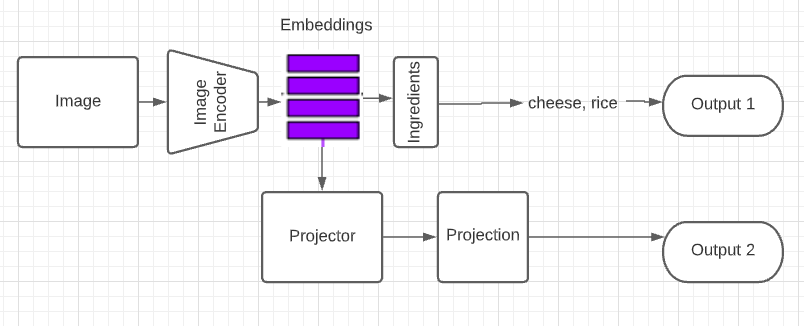
\includegraphics[width=5in]{Screenshot from 2021-12-10 18-59-47.png}
\caption{Solution Architecture}
\end{figure}
\section{Results}
We started with evaluating different pre-trained models to be used as image encoders, below is their loss on validation set. 
\begin{table}[h]
\begin{center}
\begin{tabular}{| l | l | l | l |}
\hline
Model & best loss (15 iterations) \\ \hline
eff1 & 0.0.02553 \\ \hline
eff2 & 0.0.02479 \\ \hline
eff3 & 0.0.02547\\ \hline
eff4 & 0.0.02962\\ \hline
eff5 & 0.0.02051\\ \hline
eff6 & 0.0.02440\\ \hline
eff7 & 0.0.02498\\ \hline
XCP  & 0.0.02027\\ \hline
RN50 & 0.0.01947\\ \hline
ICPV2 & 0.0.04324\\ \hline
VGG19 & 0.0.01973\\ \hline
VGG16 & 0.0.01978\\ \hline
RN101 & 0.0.01949\\ \hline
\end{tabular}
\end{center}
\caption{\label{tab:table-4}Loss with images}
\end{table}

\begin{table}[h]
\begin{center}
\begin{tabular}{| l | l | l | l |}
\hline
Model &	best loss (15 iterations)\\ \hline
eff1 & 0.0.02689\\ \hline
eff2 & 0.0.02496 \\ \hline
eff3 & 0.0.02553 \\ \hline
eff4 & 0.0.02362 \\ \hline
eff5 & 0.0.02044\\ \hline
eff6 & 0.0.01980\\ \hline
eff7 & 0.0.01969 \\ \hline
XCP &  0.0.01954 \\ \hline
RN50 & 0.0.02022 \\ \hline
\end{tabular}
\end{center}
\caption{\label{tab:table-4}Loss with 50D Glove Title embeddings + images}
\end{table}
After these experiments were performed, we made a decision to choose Resnet50 as our base model. We use these weights and trained a project to demonstrate the usability of our embeddings and results were good. Below are dishes from 4 different clusters with their ingredients included in next image. Though it is difficult to directly correlate images with ingredients (since this network does not include the weights of final layer), they look very close in terms of those.
\begin{figure}[H]
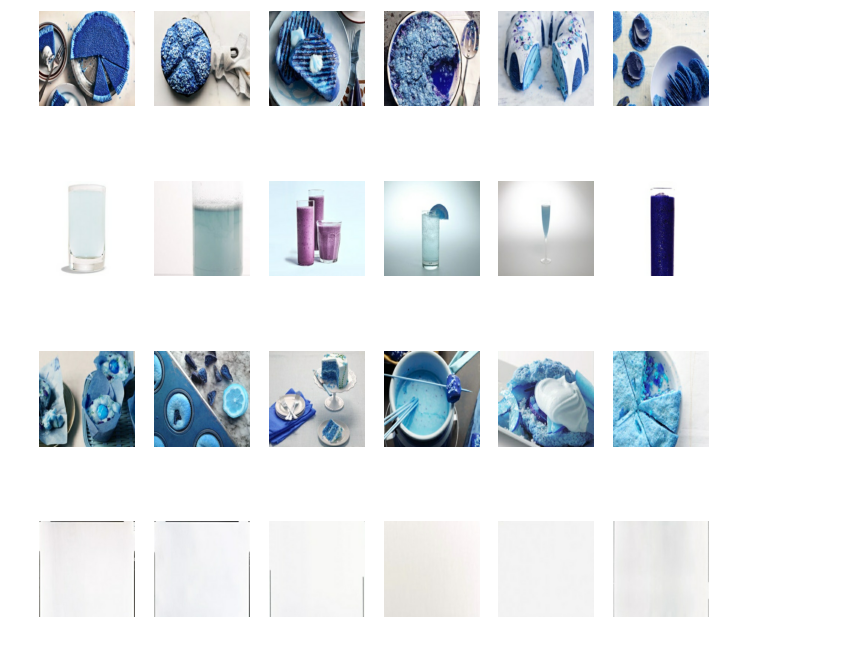
\includegraphics[width=5in]{Screenshot from 2021-12-10 22-01-07.png}
\caption{Clustering Results}
\end{figure}
\begin{figure}[H]
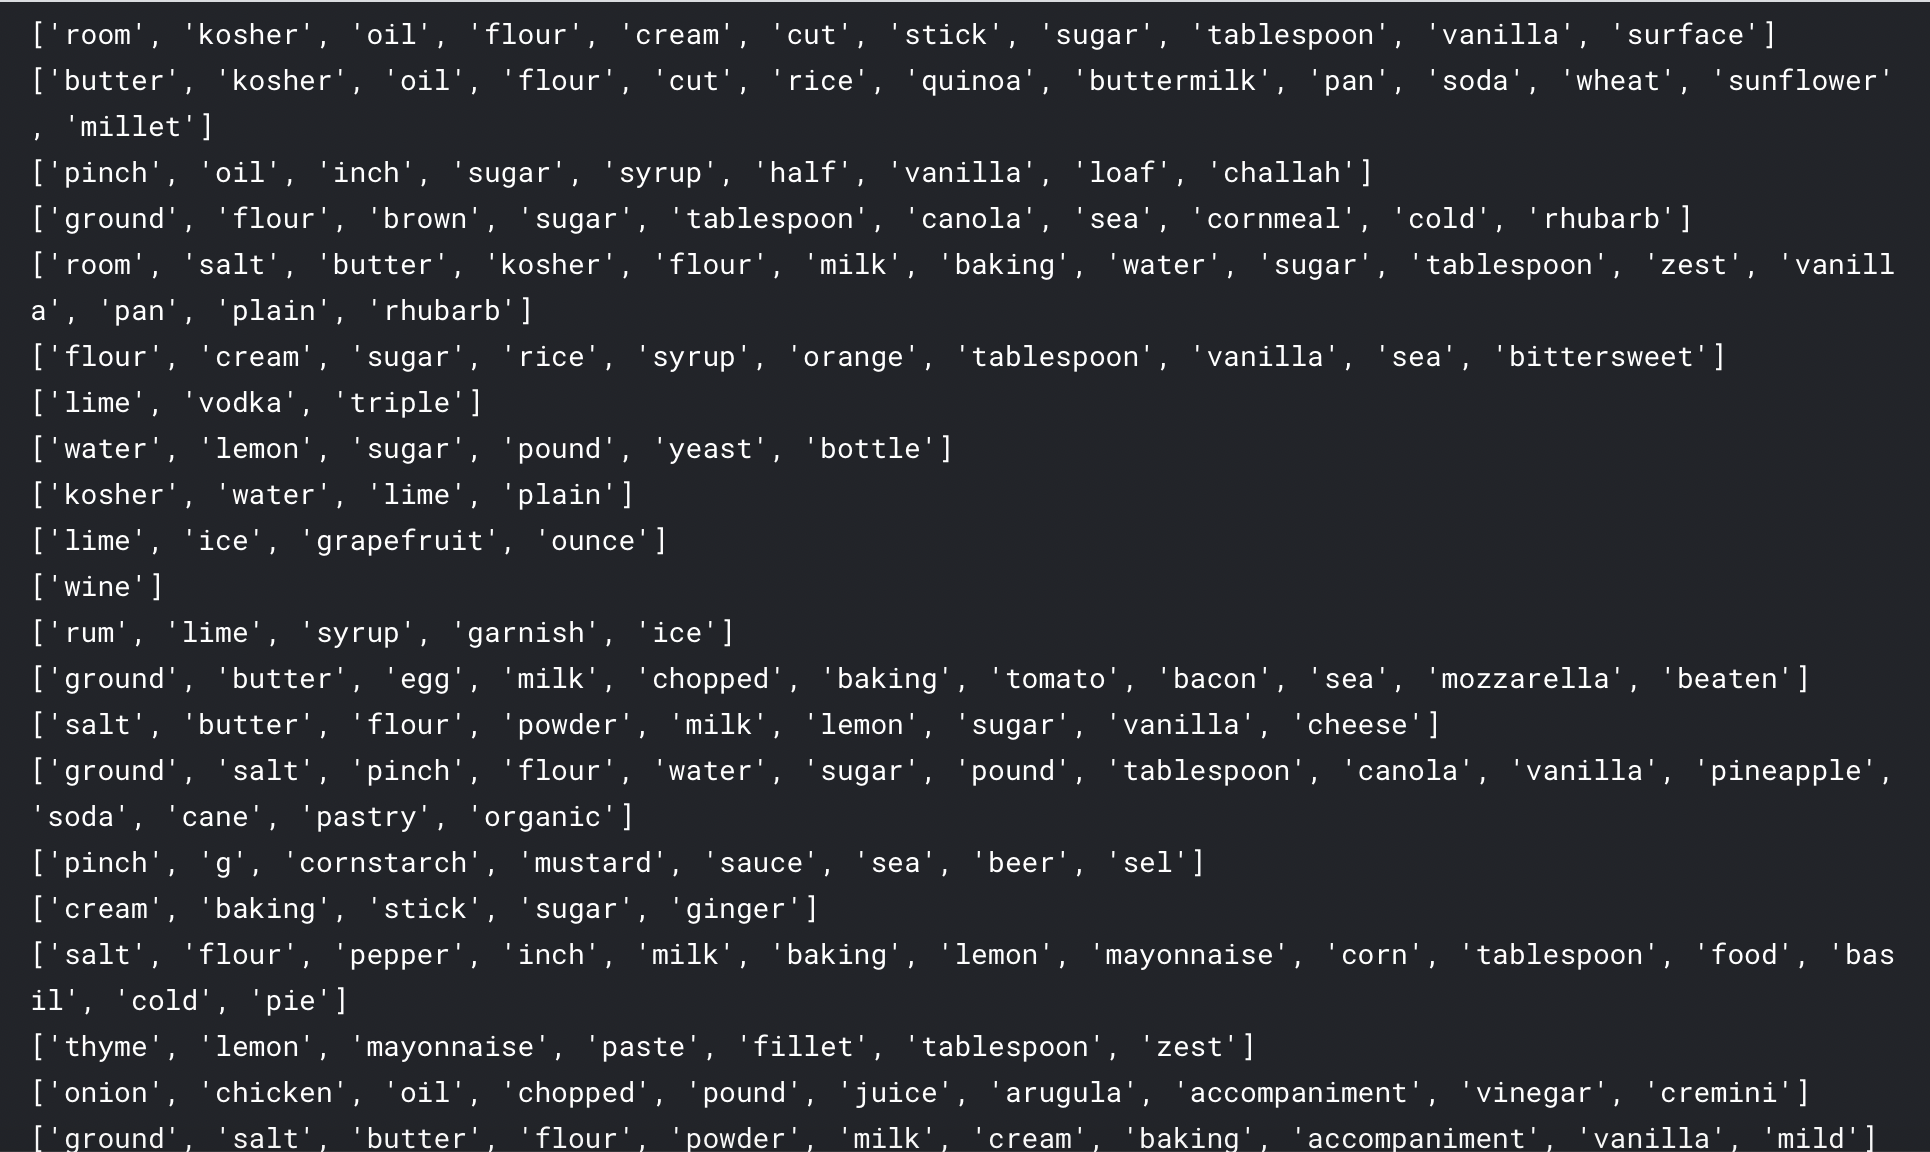
\includegraphics[width=5in]{Screen Shot 2021-12-12 at 5.38.38 PM}
\caption{Image wise Ingredients of Clustered Images}
\end{figure}
This last image shows the loss of validation set as we progress in our training.
\begin{figure}[H]
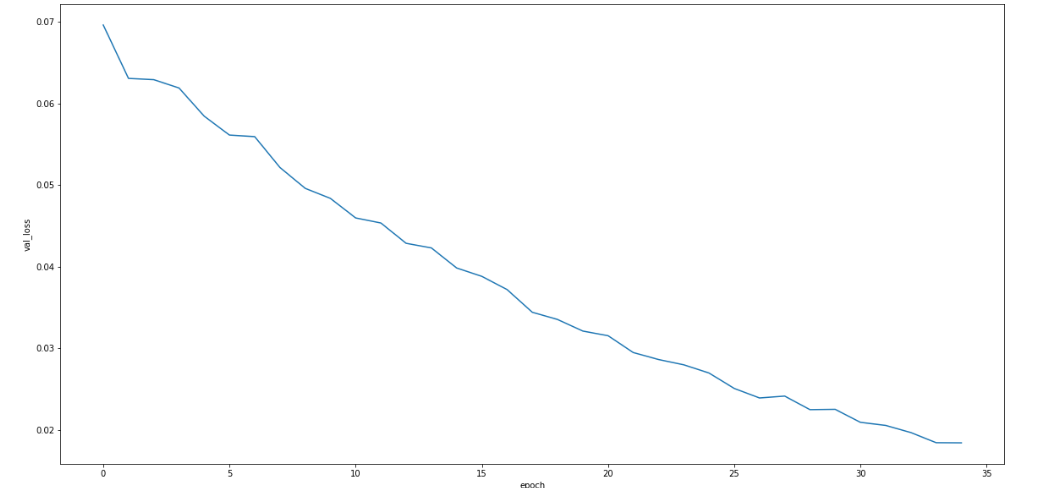
\includegraphics[width=5in]{Screenshot from 2021-12-12 18-41-44.png}
\caption{Validation Set Contrastive Loss}
\end{figure}

\section{Conclusion}
Even though classification of dishes has garnered a lot of attention in past in terms of which cuisine they belong to (probably because presence of lot of datasets) etc, we felt that there was an absence of novel work which tries to distinguish (or cluster) dishes in terms of dishes, even though the later might sound more useful and might find a lot more applications. This work tries to achieve same through a amalgamation of different techniques we learnt over the course.
Following are the final outputs of our work.

\begin{enumerate}
    \item \href{https://github.com/thunderock/DeepFoodie}{Code repository}
    \item \href{https://www.kaggle.com/alphadraco/deepfoodie}{Cleaned and semi cleaned datasets}
    \item \href{https://www.kaggle.com/alphadraco/deepfoodiedataloaders}{Final TFRecords}
\end{enumerate} 

\section{References}
\href{http://pic2recipe.csail.mit.edu}{1M+ recipe dataset} \\
\href{https://nlp.stanford.edu/projects/glove/}{Glove embeddings} \\
\href{https://arxiv.org/pdf/1812.06164.pdf}{Inverse Cooking}\\
\href{https://www.kaggle.com/carloszonetgmailcom/asthma-trigger-prediction-model-trainning}{Example to create TF records} \\
\href{https://keras.io/examples/vision/semantic_image_clustering/}{example for semantic clustering} \\

\end{document}
